\section{Modernization: Focal Loss and Temporal Graph Networks}\label{sec:modern}

The ablation study above establishes, from a single training seed, that hand-crafted topology features carry a leakage-free signal on BankSim and (conditionally) on IBM AML. Two questions remain unanswered by a single seed: whether that signal is robust to run-to-run randomness, and whether a \emph{learned} structural representation --- one that does not depend on the five hand-designed detectors --- can do better. This section reports a second, purpose-built study that answers both. Every arm below is trained with three random seeds (42, 43, 44) and reported as mean $\pm$ standard deviation, the project's own minimum bar for treating a difference as real rather than noise. Two independent upgrades to the locked XGBoost baseline are tested: (1) focal loss~\cite{lin2017focal} as an alternative to class-weighting for handling the $<$1.3\% fraud rate, implemented as a custom, deliberately alpha-free XGBoost~\cite{chen2016xgboost} objective so that it never doubles up with class weights as a second imbalance mechanism; and (2) a Temporal Graph Network (TGN)~\cite{rossi2020temporal}, a self-supervised, label-free encoder that learns a 32-dimensional GRU memory vector per account from the raw transaction stream and emits it, frozen, as 65 additional feature columns (32 source-account dimensions, 32 destination-account dimensions, and one scalar ``edge-expectedness'' score summarizing how surprising the pair is given the account's history). Because it is trained purely as next-link prediction, TGN sees no fraud labels and, following the project's own lapping-detector lesson, is deliberately amount-blind: it observes only who transacted with whom and when.

All results in this section come from \texttt{paper/data/modern.json} (the controlled multi-seed comparison) and \texttt{paper/data/final\_champions.json} (the actual champion-selection pipeline, which additionally runs a light 20-configuration hyperparameter search); numbers drawn from the single-seed ablation study are marked explicitly as such. Four feature-family arms are compared, holding the time-aware splits, XGBoost hyperparameters and (where noted) imbalance mechanism fixed within each comparison: \textbf{A} = ordinary transaction features only (21/8/20/15 features for BankSim/IBM~AML/SAP~Würzburg/synth\_erp); \textbf{B} = A + the 13 hand-crafted topology features; \textbf{C} = A + the 65 TGN columns (no hand-crafted topology); \textbf{D} = A + topology + TGN combined. The 13-feature topology block and 65-feature TGN block are identical in width across all four datasets, which is a useful internal consistency check: $|A|+13+65$ equals the reported full-feature-set size in every case (e.g.\ $21+13+65=99$ for BankSim, $8+13+65=86$ for IBM~AML). The focal-vs-class-weight comparison is run on arms A and B only (both imbalance mechanisms); arms C and D are run with class weights alone, since their purpose is to isolate the marginal value of a learned structural representation, not to re-litigate the imbalance-mechanism question a second time.

One dataset-scope note carries over from the ablation study: SAP Würzburg's splits in this section (120{,}341 / 40{,}114 / 40{,}116 train/val/test, 204/19/25 frauds, taken from \texttt{modern.json} and matching \texttt{final\_champions.json}) are the non-partition-aware split, not the partition-aware split (120{,}411 / 40{,}137 / 40{,}139) used elsewhere in this paper's headline ablation; the two SAP Würzburg number sets should not be pooled.

\subsection{Focal loss versus class weights}

Table~\ref{tab:focal-arms} reports the three-seed test PR-AUC for the ordinary-only (A) and ordinary+topology (B) arms under both imbalance mechanisms. Focal loss helps on the ordinary-only baseline in all four datasets, most dramatically on SAP Würzburg (+0.0383) and synth\_erp (+0.1690); once topology is added, its effect is mixed --- a small loss on BankSim ($-0.0060$), a wash on IBM AML (0.0000, both already at the PR-AUC ceiling), a large and volatile gain on SAP Würzburg (+0.2460, on 25 test frauds), and a solid gain on synth\_erp (+0.2014).

\begin{table}[t]
\centering
\caption{Three-seed test PR-AUC, class weights vs.\ focal loss ($\gamma{=}2.0$), ordinary-only (A) and ordinary+topology (B) arms. $\Delta$ = focal $-$ class-weight. $^\dagger$synth\_erp is synthetic and never used as thesis evidence.}
\label{tab:focal-arms}
\resizebox{\columnwidth}{!}{%
\scriptsize
\begin{tabular}{lrrrrrr}
\toprule
Dataset & A$_{cw}$ & A$_{focal}$ & $\Delta_A$ & B$_{cw}$ & B$_{focal}$ & $\Delta_B$ \\
\midrule
BankSim & 0.7870{\tiny$\pm$0.0700} & 0.8616{\tiny$\pm$0.0001} & +0.0746 & 0.9319{\tiny$\pm$0.0017} & 0.9259{\tiny$\pm$0.0008} & $-$0.0060 \\
IBM AML & 0.9920{\tiny$\pm$0.0026} & 0.9968{\tiny$\pm$0.0001} & +0.0048 & 1.0000{\tiny$\pm$0.0000} & 1.0000{\tiny$\pm$0.0000} & 0.0000 \\
SAP Würzburg & 0.1581{\tiny$\pm$0.0129} & 0.1963{\tiny$\pm$0.0252} & +0.0383 & 0.0717{\tiny$\pm$0.0095} & 0.3177{\tiny$\pm$0.1470} & +0.2460 \\
synth\_erp$^\dagger$ & 0.2483{\tiny$\pm$0.0602} & 0.4173{\tiny$\pm$0.0120} & +0.1690 & 0.4569{\tiny$\pm$0.1547} & 0.6583{\tiny$\pm$0.0031} & +0.2014 \\
\bottomrule
\end{tabular}}
\end{table}

The most consequential effect of focal loss, however, is not its mean shift but its effect on \emph{variance}. On BankSim's ordinary-only arm, moving from class weights to focal loss collapses the three-seed standard deviation from 0.0700 to 0.00007 --- roughly three orders of magnitude, from ``a coin-flip's width of uncertainty'' to ``machine-precision-adjacent.'' This is sharpened by comparing against the single-seed ablation study, which reported a BankSim baseline PR-AUC of 0.8330 (\texttt{ablation.json}, seed 42 only, class weights). That single number sits roughly two-thirds of one standard deviation above the three-seed class-weight mean of 0.7870 reported here --- a concrete illustration of why the project's own methodology treats single-seed differences smaller than $\sim$0.01 PR-AUC as noise: an unlucky or lucky seed choice alone can move the class-weighted BankSim baseline by several hundredths. Under focal loss the same arm's three-seed spread (0.8616 $\pm$ 0.00007) makes this kind of seed sensitivity essentially disappear.

This variance-collapsing property is also what wins focal loss its place in the champion pipeline. Table~\ref{tab:champion-selection} reports \texttt{final\_champions.json}'s validation-selection step, which compares the full feature set (A+B+C combined, i.e.\ arm D) under class weights against the same feature set under focal loss and selects whichever wins on validation PR-AUC --- never on test. Focal loss wins the selection on three of the four datasets: BankSim, SAP Würzburg, and synth\_erp; on IBM AML the two mechanisms tie exactly at the saturated ceiling (1.0000 vs.\ 1.0000) and the pipeline's tie-break falls to class weights. Note that this selection step differs from the controlled arm-D comparison in that it also runs a 20-configuration hyperparameter search per candidate (skipped only for SAP Würzburg, whose validation fraud count trips the pipeline's own small-sample guard), so its validation numbers are close to, but not identical with, the fixed-hyperparameter arm-D numbers reported elsewhere in this section --- for example BankSim's tuned class-weight validation PR-AUC is 0.9489 versus the fixed-hyperparameter arm D's 0.9426.

\begin{table}[t]
\centering
\caption{Champion validation selection (\texttt{final\_champions.json}), full feature set (topology+TGN+ordinary). Margin = focal $-$ class-weight on validation. $^\ddagger$selection flagged \texttt{reliable=false} (SAP Würzburg's HPO was skipped by the small-sample guard). $^\dagger$synth\_erp is non-evidentiary.}
\label{tab:champion-selection}
\resizebox{\columnwidth}{!}{%
\scriptsize
\begin{tabular}{lrrlrr}
\toprule
Dataset & Val (cw) & Val (focal) & Winner (margin) & Test (cw) & Test (focal) \\
\midrule
BankSim & 0.9489{\tiny$\pm$0.0009} & 0.9515{\tiny$\pm$0.0007} & focal (+0.0026) & 0.9395{\tiny$\pm$0.0006} & 0.9364{\tiny$\pm$0.0015} \\
IBM AML & 1.0000{\tiny$\pm$0.0000} & 1.0000{\tiny$\pm$0.0000} & cw (tie, 0.0000) & 1.0000{\tiny$\pm$0.0000} & 1.0000{\tiny$\pm$0.0000} \\
SAP Würzburg & 0.2888{\tiny$\pm$0.0436} & 0.3562{\tiny$\pm$0.0195} & focal$^\ddagger$ (+0.0674) & 0.1401{\tiny$\pm$0.0076} & 0.1557{\tiny$\pm$0.0717} \\
synth\_erp$^\dagger$ & 0.8487{\tiny$\pm$0.0017} & 0.8507{\tiny$\pm$0.0025} & focal (+0.0020) & 0.7722{\tiny$\pm$0.0014} & 0.7785{\tiny$\pm$0.0053} \\
\bottomrule
\end{tabular}}
\end{table}

BankSim deserves a specific flag: its validation margin, +0.0026 PR-AUC, is the thinnest \emph{reliable, non-saturated, real-data} margin in the entire selection table --- synth\_erp's nominal margin (+0.0020) is numerically smaller but is excluded from thesis claims as synthetic data, and IBM AML's margin is a literal zero-width tie on an already-saturated metric, not a genuine comparison. A margin this thin, on the dataset the project treats as its cleanest structural-signal testbed, does not survive contact with the test set: the class-weight arm actually scores higher on BankSim's held-out test period (0.9395 $\pm$ 0.0006) than the focal arm that was selected on validation (0.9364 $\pm$ 0.0015), a reversal of 0.0032 PR-AUC. We report this plainly as a caution against over-reading small validation margins, per the project's own threshold-freezing discipline; it does not overturn the selection (validation-only selection is the whole point of never touching test until after the choice is frozen), and it is operationally invisible at the metric an auditor actually cares about --- precision@100 is 1.00 for both arms.

\subsection{Temporal graph network embeddings}

Table~\ref{tab:tgn-lift} isolates the value of the learned TGN representation against two references: the ordinary-only baseline (arm C $-$ arm A, both class-weighted) and the hand-crafted topology block (arm C $-$ arm B), plus the incremental value of combining both representations (arm D $-$ arm B) and TGN's share of total SHAP feature importance in the champion model (from \texttt{final\_champions.json}'s per-dataset SHAP summary).

\begin{table}[t]
\centering
\caption{TGN embeddings vs.\ hand-crafted topology, 3-seed test PR-AUC deltas (class-weighted arms only) and TGN's share of total SHAP importance in the champion model. $^\dagger$synth\_erp is non-evidentiary.}
\label{tab:tgn-lift}
\resizebox{\columnwidth}{!}{%
\scriptsize
\begin{tabular}{lrrrr}
\toprule
Dataset & TGN$-$base. & TGN$-$topo. & Comb.$-$topo. & TGN SHAP share \\
\midrule
BankSim & +0.1326 & $-$0.0123 & +0.0004 & 17.5\% \\
IBM AML & $-$0.0048 & $-$0.0128 & 0.0000 & 1.9\% \\
SAP Würzburg & $-$0.0987 & $-$0.0124 & +0.0684 & 42.0\% \\
synth\_erp$^\dagger$ & +0.4489 & +0.2404 & +0.2850 & 37.3\% \\
\bottomrule
\end{tabular}}
\end{table}

The central, load-bearing finding of this table is the middle column. On every real dataset, TGN alone (arm C) scores \emph{below} hand-crafted topology alone (arm B): $-$0.0123 on BankSim, $-$0.0128 on IBM AML, $-$0.0124 on SAP Würzburg. These three deltas are remarkably tight given how different the three datasets are in scale, fraud rate, and graph density --- all three cluster within 0.0005 of $-$0.0125. Learned, self-supervised structural embeddings simply do not beat five purpose-built, domain-informed detectors on real transaction graphs in this study; the only dataset where TGN outperforms hand-crafted topology is synth\_erp (+0.2404), the project's own synthetic environment, which is explicitly excluded from evidentiary claims (Section~\ref{sec:threats}). The first column tells a related but distinct story: TGN's lift over the plain ordinary-feature baseline is positive on BankSim (+0.1326, nearly matching topology's own +0.1449 lift there) but slightly \emph{negative} on both IBM AML ($-$0.0048) and SAP Würzburg ($-$0.0987). On IBM AML this is a small movement within noise (both arms sit near the saturated ceiling, std $\approx$0.01); on SAP Würzburg it is a large, consistent penalty, echoing the same dataset's negative topology lift reported in the ablation study --- on this small, thin ERP ledger, adding structural feature complexity of either kind tends to hurt rather than help, plausibly because 25 test frauds cannot support the additional degrees of freedom either representation introduces.

Combining topology and TGN (arm D vs.\ arm B) adds negligible value beyond topology alone on the two datasets with the cleanest signal: +0.0004 on BankSim, 0.0000 on IBM AML (already saturated). SAP Würzburg's combined arm does show a nominal +0.0684 recovery over its topology-only arm, but this sits inside the same small-sample volatility that produced SAP's other large, sign-flipping deltas in this section and should not be read as evidence that TGN rescues topology's failure there. synth\_erp's large combined gain (+0.2850) is, again, a synthetic-data result only.

A last observation cautions against reading SHAP importance share as a proxy for ablation-validated value. SAP Würzburg's TGN block claims the \emph{largest} share of total SHAP importance of any dataset in this study (42.0\%) despite producing the study's most negative TGN lift ($-$0.0987 over baseline, $-$0.0124 over topology); IBM AML shows the opposite pattern, with TGN carrying almost no importance (1.9\%) on a baseline it also fails to improve. A feature family can dominate a model's internal attribution and still not earn its place in a leakage-free ablation --- the same lesson the ablation study draws for hand-crafted cycle features applies here to a learned representation as well, via TreeSHAP's exact per-feature attribution~\cite{lundberg2017unified,lundberg2020local}.

%% FIGURE TODO: grouped bar chart, one group per dataset (BankSim, IBM AML, SAP Würzburg, synth_erp), two bars per group showing tgn_vs_handcrafted_topology and combined_vs_topology (PR-AUC delta, signed, with a zero reference line), to make visually obvious that the "TGN vs topology" bar is negative on all three real datasets and positive only on synth_erp.
\begin{figure}[t]
\centering
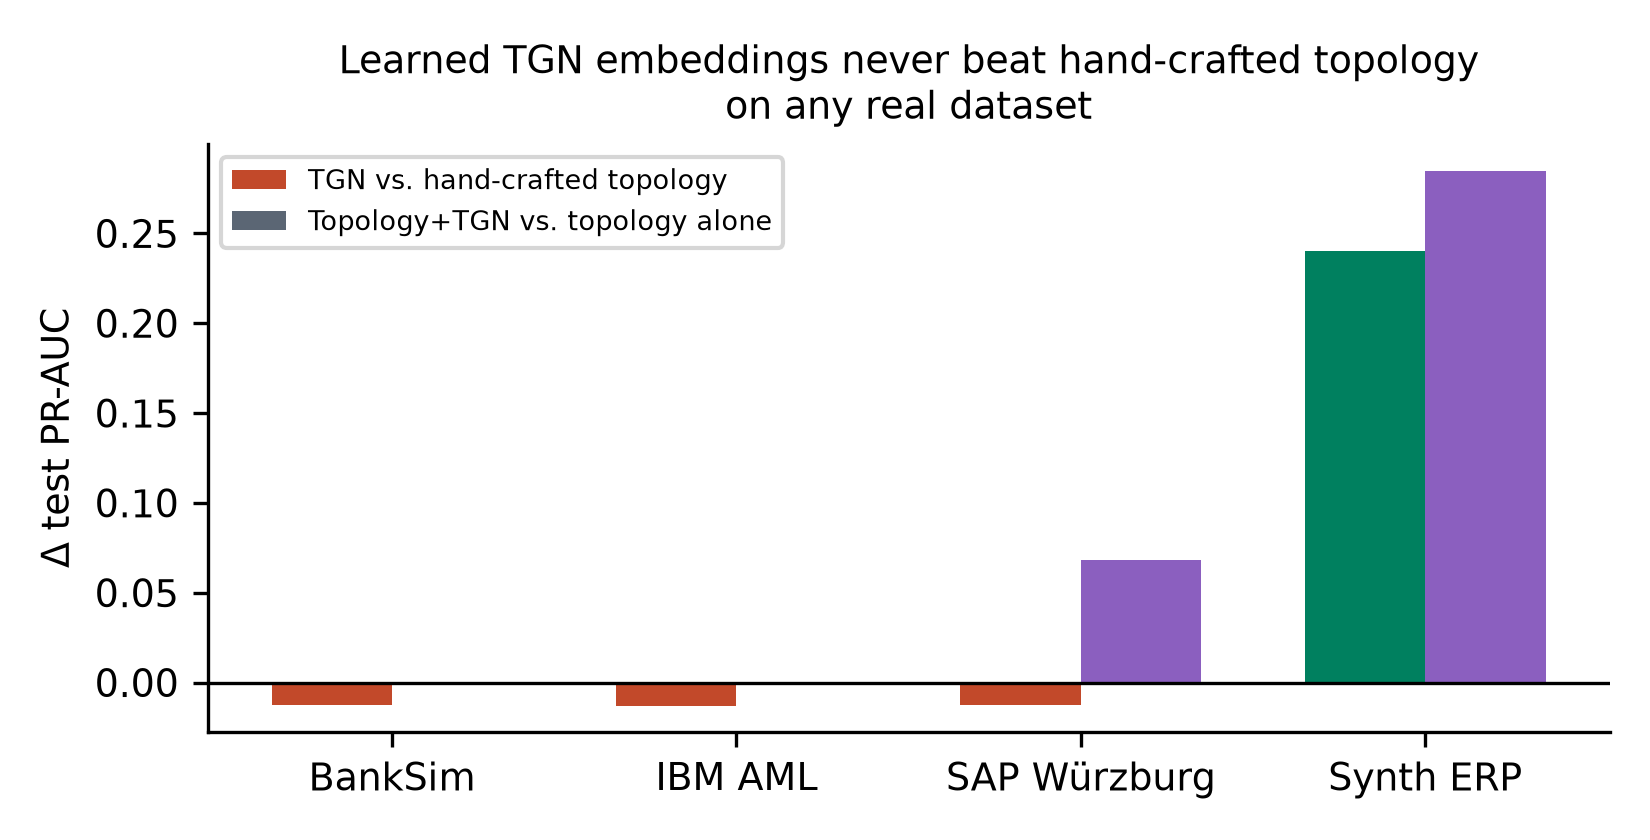
\includegraphics[width=\columnwidth]{figures/modern_tgn_lift_by_dataset.png}
\caption{TGN-vs-topology and combined-vs-topology PR-AUC deltas by dataset (\texttt{modern.json}). The TGN-vs-topology bar is negative on all three real datasets and positive only on the non-evidentiary synth\_erp dataset.}
\label{fig:tgn-lift}
\end{figure}

\subsection{Implication for the production system}

Two independent findings close off TGN as a candidate for the served model, both already on the record from this build. First, TGN training is not bit-reproducible across machines even with a fixed seed: re-running the TGN trainer on freshly downloaded copies of the same source data and re-scoring against the committed champion bundle does not reproduce the committed test PR-AUC --- BankSim recomputes to 0.845 against the bundle's recorded 0.938, and SAP Würzburg to 0.098 against the bundle's 0.140 (Section~\ref{sec:threats}, Threats to Validity). Small floating-point differences in CPU-side PyTorch training compound across epochs and propagate through a feature block that carries 17--42\% of the champion model's total SHAP importance (Table~\ref{tab:tgn-lift}), so an offline champion bundle trained on one machine cannot be assumed to reproduce its recorded score on another. Second, and independently disqualifying, the TGN's per-account GRU memory tensor --- the running state that makes its embeddings meaningful at any given point in time --- is never persisted by the training code; it exists only inside the training process and is discarded on exit, so there is no artifact from which a live scoring service could resume the memory a freshly arriving transaction would need.

For these reasons, the production system described in Section~\ref{sec:production} does not serve the TGN-augmented champion at all. It serves a separate, explicitly named \emph{online} bundle --- ordinary features plus hand-crafted topology only, arm B's feature set --- built and reported independently in \texttt{paper/data/online\_bundles.json}: 34 features and test PR-AUC 0.9311 $\pm$ 0.0005 on BankSim, 33 features and 0.1094 $\pm$ 0.0198 on SAP Würzburg, and 28 features and 0.5702 $\pm$ 0.0174 on synth\_erp. IBM AML's online-bundle entry, labeled \texttt{ibm\_aml\_kaggle} (26 features, test PR-AUC 0.5120 $\pm$ 0.0674), is a fresh Kaggle re-download reproduction check, not the same simulator instance behind this section's headline IBM AML numbers, and its PR-AUC is correspondingly far below this section's saturated 1.0000 --- a difference of instance, not of method, and one more reason the two IBM AML number sets in this paper must never be merged. In short: every PR-AUC reported in this section for the ``champion'' or ``combined'' arm describes an offline, research-only model; the number that describes what a live transaction would actually be scored against is the online-bundle figure above, and it excludes TGN entirely.
